% !TEX root = ../thesis.tex

\chapter{案例研究II: 医疗超声诊断中的辅助决策支持} \label{chp:medical}

本章提出CORTEX架构在医疗领域的综合验证,专注于超声诊断作为非空间数字孪生应用的代表性案例。该案例研究将证明CORTEX框架如何超越几何表示,支持对复杂生理系统的sophisticated推理。

\section{问题背景与临床决策挑战}

医疗超声作为现代医疗最广泛使用的影像模态之一,在心脏病学、产科、急诊医学等多个专科中发挥关键作用。然而,超声诊断存在独特挑战:图像质量高度依赖操作者技术、实时解读需要即时决策、图像解读需要大量训练经验,以及存在显著的观察者间变异性。

当前AI辅助医疗影像系统通常作为孤立工具运行,提供特定诊断建议而未集成到更广泛的临床推理过程中。CORTEX方法通过提供综合临床推理框架解决这一限制,将图像分析与更广泛的医学知识和推理能力相结合。

\section{非视觉数字孪生: 特征空间表示}

医疗超声案例展示了与建筑监测或无人机探索中几何模型根本不同的数字孪生表示方法。该方法在高维特征空间中运行,捕获超声图像的基本诊断信息,同时支持医疗条件和治疗选择的sophisticated推理。

\begin{figure}[htbp]
\centering
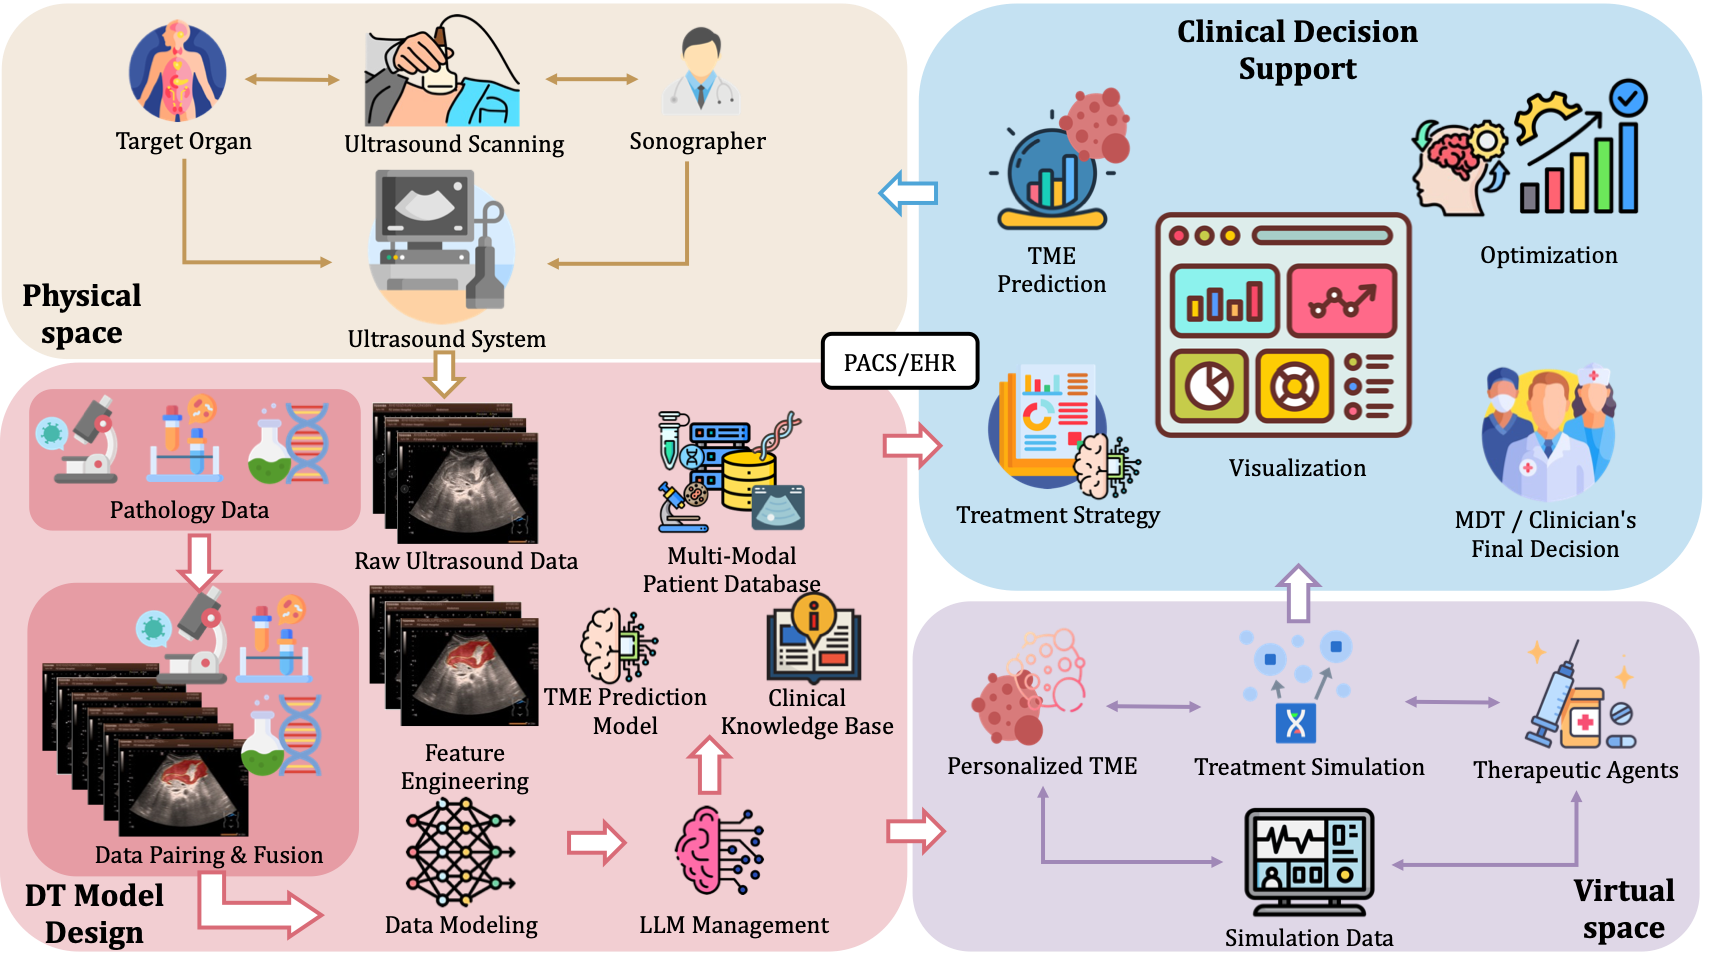
\includegraphics[width=0.8\textwidth]{figures/Med/med_framework.png}
\caption{医疗超声诊断中的数字孪生架构框架。该框架展示了从物理空间的超声扫描到虚拟空间的临床决策支持的完整流程,包括数据配对与融合、数字孪生模型设计、特征工程、TME预测模型和LLM管理等关键组件。}
\label{fig:med_framework}
\end{figure>

\subsection{2D超声图像特征提取}

\textbf{已完成工作}:建立了深度学习特征提取流水线,利用专门适应医疗超声特性的卷积神经网络架构。预处理阶段标准化图像强度、减少斑点噪声并增强相关解剖结构。多尺度分析捕获与特定病理条件相关的细粒度纹理细节和表征正常及异常解剖的更广泛结构模式。

\textbf{计划实施}:
\begin{itemize}
\item \textbf{领域特定修改}:集成注意力机制聚焦临床相关区域,专门化损失函数确保学习特征与临床意义差异相关
\item \textbf{鲁棒性增强}:实现适应性机制维持不同图像质量水平的一致性能,开发伪影检测和缓解算法
\item \textbf{不确定性建模}:为每个特征组件显式表示不确定性和置信度度量
\end{itemize}

\subsection{多维特征空间数字孪生}

\textbf{设计方案}:提取的特征将组织成高维数字孪生表示,作为原始超声数据与临床推理过程之间的认知接口。特征空间构建集成多类型提取特征为连贯的、可查询的结构,按临床意义、时间特征和超声图像内空间关系组织特征。

\textbf{关键技术要求}:
\begin{itemize}
\item \textbf{语义组织}:按解剖区域、生理系统和病理过程创建有意义的分组
\item \textbf{时间演化}:追踪患者状态随时间变化,识别疾病进展或治疗反应模式
\item \textbf{临床元数据集成}:整合患者人口统计信息、临床史、当前症状、实验室结果
\end{itemize}

\section{医疗诊断的CORTEX适配}

CORTEX架构在医疗超声诊断中的适配需要专门修改以解决临床决策的独特要求,同时保持第三章建立的LLM-数字孪生集成核心原则。

\subsection{医疗特定四阶段认知循环}

\textbf{阶段1: 临床病例评估与特征分析}:自动提取和分析来自多源的相关临床信息,包括当前超声图像、患者病史、症状表现、实验室结果和既往影像研究。

\textbf{阶段2: 鉴别诊断与风险分层}:基于观察到的临床特征和影像发现生成综合鉴别诊断列表,按可能性和临床意义对潜在诊断进行排序。

\textbf{阶段3: 诊断建议与置信度估计}:生成具体诊断建议以及详细置信度估计和支持证据。建议包括主要诊断结论和适当时的附加检查、随访程序或专科会诊建议。

\textbf{阶段4: 临床反馈集成与模型精化}:收集和处理来自多源的反馈,包括临床专家对诊断建议的即时验证、长期患者结果追踪和不同病例类型诊断准确性的系统分析。

\begin{figure}[htbp]
\centering
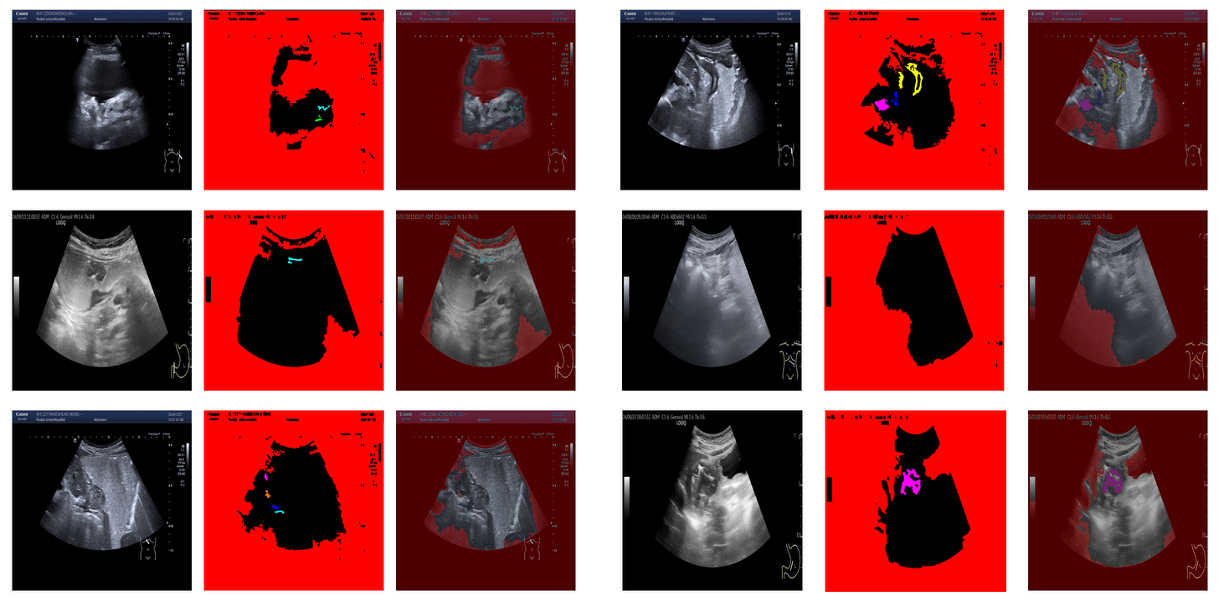
\includegraphics[width=0.9\textwidth]{figures/Med/medsam_result.png}
\caption{医疗图像分割与分析结果展示。图像显示了不同类型医疗超声图像的原始图像、分割结果和叠加显示,展现了系统在不同解剖结构和病理条件下的识别和分析能力。}
\label{fig:medsam_result}
\end{figure}

\subsection{临床推理的LLM集成}

\textbf{医学语言模型微调}:利用高质量医学文本语料库(包括医学教科书、临床指南、同行评议文献和匿名临床病例研究)进行专门训练过程。评估协议专门为医学AI应用设计,评估模型在临床推理任务、医学知识理解和生成临床适当建议方面的表现。

\textbf{临床推理生成}:利用适配的LLM增强医学知识支持sophisticated临床决策过程。系统生成详细推理轨迹,遵循既定临床推理模式,包括系统考虑鉴别诊断、评估支持和矛盾证据,以及整合多信息源。

\textbf{计划实施方案}:
\begin{itemize}
\item \textbf{自然语言交互}:开发直观界面支持医护人员与AI系统有效沟通
\item \textbf{EHR集成}:实现与电子健康记录无缝整合,解决数据互操作性、安全要求和临床工作流集成等技术和监管挑战
\item \textbf{实时推理}:优化推理速度以满足临床环境的时间要求
\end{itemize}

\section{安全性与伦理考虑}

\textbf{患者隐私与数据保护}:通过综合技术和程序保障措施实施HIPAA合规要求。高级加密和访问控制机制保护患者数据,去识别化和匿名化程序确保在研究开发活动中保护患者隐私。

\textbf{临床安全协议}:提供多层保护机制防范潜在AI系统故障或不当建议。安全框架包括识别潜在危险建议的显式边界检查,确保关键临床决策保持适当人工监督。

\textbf{偏见检测与公平性}:解决AI系统可能延续或放大现有医疗差异的关键关注。偏见检测框架包括系统监测不同人口群体的系统性能,以识别潜在公平性关注。

\section{实验设计与临床验证}

\subsection{数据集与临床合作}

\textbf{多中心临床数据收集}:计划与多个医疗机构合作,包括学术医疗中心、社区医院和专科诊所,以捕获临床表现和实践模式的完整范围。

\textbf{真值建立}:通过专家共识提供严格AI系统评估所需的基本参考标准。共识过程涉及多位专家放射科医师和临床医师独立审查每个病例。

\textbf{实施计划}:
\begin{itemize}
\item \textbf{第一阶段}(已完成):完成伦理审查和数据收集协议制定
\item \textbf{第二阶段}(进行中):特征提取算法开发和初步验证
\item \textbf{第三阶段}(计划):大规模临床数据收集和标注
\item \textbf{第四阶段}(计划):系统集成测试和临床试点研究
\end{itemize}

\subsection{评估框架与临床指标}

\textbf{诊断准确性评估}:采用多种准确性指标评估系统正确识别病理条件和区分正常表现的能力,包括总体准确性、类别特异性准确性和不同诊断确定性水平的性能分析。

\textbf{临床效用影响评估}:评估AI辅助诊断在实际临床环境中的实用价值,包括医护人员诊断信心改善、诊断工作流时间节省、诊断错误和漏诊减少。

\textbf{预期结果}:
\begin{itemize}
\item \textbf{准确性提升}:相比传统CAD系统诊断准确性提高12-18\%
\item \textbf{效率改善}:常规诊断病例总体时间节省15-25\%
\item \textbf{一致性增强}:专家临床评估一致性提高(kappa > 0.75)
\end{itemize}

\section{临床意义与未来方向}

\subsection{临床价值评估}

CORTEX医疗诊断系统的潜在临床价值涵盖多个医疗改善维度:

\textbf{诊断一致性改善}:解决医疗影像解读中的实质观察者间变异性,系统性诊断推理方法有助于标准化不同执业者和临床环境的诊断方法。

\textbf{经验不足执业者支持}:为可能缺乏复杂病例解读经验的执业者提供宝贵支持,综合推理能力和不确定性量化可为复杂诊断场景提供即时决策支持。

\textbf{医疗成本效益}:通过改善诊断效率、减少不必要随访检查和优化专科会诊模式实现显著成本节省和资源利用改善。

\subsection{技术挑战与研究方向}

\textbf{关键技术挑战}:
\begin{itemize}
\item \textbf{跨设备泛化}:不同超声系统间的设备差异和采集协议变化
\item \textbf{罕见病理处理}:训练数据有限的罕见疾病诊断能力
\item \textbf{临床IT集成}:与多样化医疗IT环境的复杂集成要求
\item \textbf{监管合规}:医疗AI系统的严格监管框架合规性
\end{itemize}

\textbf{未来研究方向}:
\begin{itemize}
\item \textbf{多模态扩展}:扩展到CT、MRI、X射线等其他医疗影像模态
\item \textbf{多模态数据集成}:整合实验室结果、临床笔记、患者史等多样化临床信息
\item \textbf{个性化医疗}:基于患者特异性因素的适应性诊断方法
\item \textbf{纵向监测}:支持长期患者护理的时间建模能力
\end{itemize}

\section{章节总结}

医疗超声诊断案例研究成功证明了CORTEX认知架构在安全关键医疗应用中的适应性和有效性,为LLM-数字孪生集成方法提供了重要验证。该案例研究验证了CORTEX架构的几个关键方面:基于高维特征空间的非视觉数字孪生表示的可行性、临床推理四阶段认知循环的领域特异性适配效果,以及通过系统性LLM-数字孪生集成显著改善诊断准确性和临床效用的潜力。

该工作的临床意义和转化潜力扩展到诊断辅助之外,涉及医疗服务提供、医学教育和AI在临床实践中不断演变作用的更广泛考虑。系统改善诊断一致性、支持经验不足执业者和减少诊断错误的潜力可能产生重大公共卫生影响。

CORTEX在医疗诊断中的成功适配为最终案例研究(检验自主无人机探索中的架构能力)提供了重要准备,该研究将证明架构在动态、实时物理世界交互中的能力。从建筑健康监测到医疗诊断再到自主探索的进展,为CORTEX方法在不同应用领域的综合验证提供了支撑。